\documentclass[11pt,a4paper]{article}
\usepackage[T1]{fontenc}
\usepackage[utf8]{inputenc}
\usepackage[provide=*,french]{babel}
\usepackage{lmodern,eurosym,enumitem,graphicx,xcolor,fancyhdr}
\usepackage[margin=17mm,top=15mm,bottom=19mm]{geometry}
\definecolor{bleu}{RGB}{50,100,205}
\pagestyle{fancy}\fancyhf{}\renewcommand{\headrulewidth}{0pt}
\fancyfoot[L]{\scriptsize mathsgo.re · CC BY-NC-SA 4.0}\fancyfoot[R]{\small\thepage}
\setlength{\parindent}{0pt}\setlength{\parskip}{5pt}
\setlist[itemize]{leftmargin=5mm,label=\textemdash,itemsep=3pt,topsep=4pt,parsep=0pt}
\newcommand{\mission}[1]{\par\medskip\noindent\colorbox{bleu}{\parbox{\dimexpr\linewidth-2\fboxsep}{\color{white}\bfseries\strut #1}}\par\smallskip}
\newcommand{\niveau}[1]{\par\medskip{\bfseries #1}\par}
\begin{document}
{\Large\bfseries Les pourcentages : missions et enquêtes}\par
\textit{Rédige tes recherches, tes calculs et tes réponses sur ton cahier.}
\mission{Mission 1 et mission 1 bis : Le travail de détective}
Des élèves ont dessiné des schémas, mais ont oublié leurs énoncés ! Pour chaque schéma, invente une histoire qui lui correspond en utilisant les pourcentages. Pose une question, puis réponds-y en expliquant ton calcul. Pour C et C bis, choisis une donnée numérique cohérente avec ton histoire.

\begin{minipage}[t]{0.48\linewidth}\textbf{En classe : mission 1}

\textbf{Enquête A}\par\centering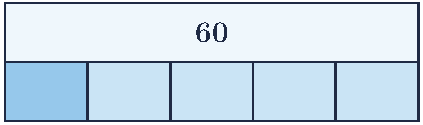
\includegraphics[page=1,width=0.88\linewidth]{diagrammes.pdf}

\raggedright\textbf{Enquête B}\par\centering\includegraphics[page=2,width=0.88\linewidth]{diagrammes.pdf}

\raggedright\textbf{Enquête C}\par\centering\includegraphics[page=3,width=\linewidth]{diagrammes.pdf}
\end{minipage}\hfill
\begin{minipage}[t]{0.48\linewidth}\textbf{À la maison : mission 1 bis}

\textbf{Enquête A bis}\par\centering\includegraphics[page=4,width=0.81\linewidth]{diagrammes.pdf}

\raggedright\textbf{Enquête B bis}\par\centering\includegraphics[page=5,width=0.88\linewidth]{diagrammes.pdf}

\raggedright\textbf{Enquête C bis}\par\centering\includegraphics[page=6,width=\linewidth]{diagrammes.pdf}
\end{minipage}

\mission{Mission 2 : Le grand piège des vendeurs}
Le 1\textsuperscript{er} mars, le gérant d'un magasin de vélos augmente tous ses prix de \textbf{20~\%}. Un mois plus tard, il annonce une réduction de \textbf{20~\% sur les prix augmentés} et affirme : « Les prix sont revenus à leur valeur de départ ! »

\textbf{Le gérant a-t-il raison ? Prouve ta réponse.}

\textit{Si besoin, choisis un prix de départ, par exemple 100~\euro{} ou 500~\euro{}, et représente les deux étapes.}
\newpage
\mission{Mission 3 : Trois problèmes pour chercher}


Pour chaque problème, explique ton raisonnement et présente les calculs utiles. Tu peux utiliser un schéma.

\niveau{\(\star\) Problème 1 : Le budget du cadeau}
Un casque coûte \textbf{80~\euro{}}. Il bénéficie d'une réduction de \textbf{25~\%}. La livraison coûte \textbf{6~\euro{}} et ne bénéficie pas de la réduction. Inès dispose de \textbf{65~\euro{}}.

\textit{Peut-elle commander ce casque ? Justifie ta réponse.}

\medskip
\niveau{\(\star\star\) Problème 2 : La randonnée}
Une randonnée fait \textbf{12~km}. Le matin, un groupe parcourt \textbf{35~\% de la distance totale}. L'après-midi, il parcourt encore \textbf{40~\% de la distance totale}.

Lina affirme qu'il reste moins de 2~km à parcourir.

\textit{A-t-elle raison ? Justifie ta réponse.}

\medskip
\niveau{\(\star\star\star\) Problème 3 : Acheter plus pour payer moins ?}
Nora veut acheter un \textbf{sac à 40~\euro{}} et une \textbf{trousse à 12~\euro{}}.

Le magasin accorde une \textbf{réduction de 20~\% sur la totalité du panier} dès que son montant, avant réduction, atteint \textbf{60~\euro{}}.

À la caisse, le vendeur lui propose d'ajouter un \textbf{carnet à 8~\euro{}} pour payer moins cher.

\textit{Le conseil du vendeur est-il avantageux pour Nora ? Justifie ta réponse.}


\mission{Mission 3 bis : Le défi des deux barres}
\niveau{\(\star\) Le jeu vidéo}
Dans un jeu de rôle, le personnage d'Alice possède \textbf{25~\% de points de magie en plus} que celui de Bob. À eux deux, ils réunissent \textbf{900 points de magie}.

\textit{Combien de points possède Bob ? Combien en possède Alice ?}

\niveau{\(\star\star\) Le collège}
Dans un collège, il y a \textbf{20~\% de filles de moins que de garçons}. Au total, il y a \textbf{450 élèves}.

\textit{Combien y a-t-il de garçons ? Combien y a-t-il de filles ?}

\textit{Si besoin, représente les deux quantités par des barres découpées en parts égales.}
\newpage
\mission{Mission 4 : Le choix du consommateur (Les t-shirts)}


Tu achètes \textbf{3 t-shirts identiques}. Leur prix avant promotion est de \textbf{20~\euro{} l'unité}, sauf indication contraire. Dans chaque magasin, seule l'offre décrite s'applique.

Pour chaque niveau, compare les offres et justifie tes réponses. Tu peux utiliser des schémas en barres.

\niveau{\(\star\) Niveau 1 : Le duel simple}
\begin{itemize}
\item \textbf{Magasin A :} Pour 2 t-shirts achetés, le troisième est offert.
\item \textbf{Magasin B :} Réduction de 30~\% sur le prix total des 3 t-shirts.
\end{itemize}
\textit{Quel magasin choisis-tu ?}

\bigskip
\niveau{\(\star\star\) Niveau 2 : La comparaison à trois}
\begin{itemize}
\item \textbf{Magasin C :} Le premier t-shirt est au prix normal ; le deuxième bénéficie de 50~\% de réduction et le troisième de 70~\% de réduction.
\item \textbf{Magasin D :} Une remise immédiate de 15~\euro{} est déduite du prix total des 3 t-shirts.
\item \textbf{Magasin E :} Chaque t-shirt bénéficie de 25~\% de réduction.
\end{itemize}
\textit{Classe ces magasins du moins cher au plus cher. Signale les éventuelles égalités.}

\bigskip
\niveau{\(\star\star\star\) Niveau 3 : Le boss des soldes}
\begin{itemize}
\item \textbf{Magasin F :} Réduction de 20~\% sur chaque t-shirt, puis réduction supplémentaire de 10~\% en caisse sur le montant déjà réduit.
\item \textbf{Magasin G :} Ici, le prix avant promotion est de \textbf{22~\euro{} par t-shirt}. Pour 2 t-shirts achetés au prix normal, le troisième coûte 1~\euro{}.
\end{itemize}
\textit{1. Quel magasin est le moins cher ? Justifie avec tes calculs.}

\textit{2. Léa affirme que l'offre F revient à enlever 30~\% du prix initial du panier. A-t-elle raison ? Justifie ta réponse.}

\newpage
\mission{Mission 5 : Taux de réduction et prix initial}


\textbf{Une nouvelle enquête :} cette fois, tu dois retrouver un pourcentage de réduction ou un prix avant réduction. Pour chaque question, explique ta démarche. Tu peux utiliser un schéma en barres ou un tableau de proportionnalité.

\niveau{\(\star\) Partie A : Retrouver le taux de réduction}
\begin{enumerate}[leftmargin=6mm,itemsep=11pt]
\item Un sac coûtait \textbf{80~\euro{}}. Il coûte maintenant \textbf{60~\euro{}}.\newline
Quel est le montant de la réduction ? Quel pourcentage du prix initial représente-t-il ?
\item Trois t-shirts coûtaient au total \textbf{60~\euro{}}. Après promotion, tu paies \textbf{36~\euro{}}.\newline
Quel est le pourcentage de réduction sur le prix total initial ?
\item Une console coûtait \textbf{400~\euro{}}. Son prix final est \textbf{308~\euro{}}.\newline
Quel est le pourcentage de réduction par rapport au prix initial ?
\end{enumerate}
\textit{Point de vigilance : pour chaque calcul, indique le prix qui représente 100~\%.}

\bigskip
\niveau{\(\star\star\) Partie B : Retrouver le prix initial}
\begin{enumerate}[leftmargin=6mm,itemsep=11pt]
\item Après une réduction de \textbf{25~\%}, un vêtement coûte \textbf{60~\euro{}}.\newline
Quel était son prix avant réduction ?
\item Après une réduction de \textbf{20~\%}, des chaussures coûtent \textbf{72~\euro{}}.\newline
Quel était leur prix avant réduction ?
\item Après une réduction de \textbf{30~\%}, une console coûte \textbf{280~\euro{}}.\newline
Quel était son prix avant réduction ?
\end{enumerate}
\textit{Pour vérifier chaque réponse, applique la réduction au prix initial que tu as trouvé. Tu dois retrouver le prix payé.}

\bigskip
\textbf{Le débat :} Pour la première question de la partie B, Sami propose d'ajouter 25~\% à 60~\euro{}. Sa méthode permet-elle de retrouver le prix initial ? Justifie avec des calculs.


\end{document}